%=============================--A--=============================%
\subsection{Módulo 4 $\pmb \mapsto$ \textit{Dematrixing} e reprodução sonóra de $L$ e $R$}
\label{subsec:mod4}

%\iffalse
\begin{figure}[H]
    \centering
    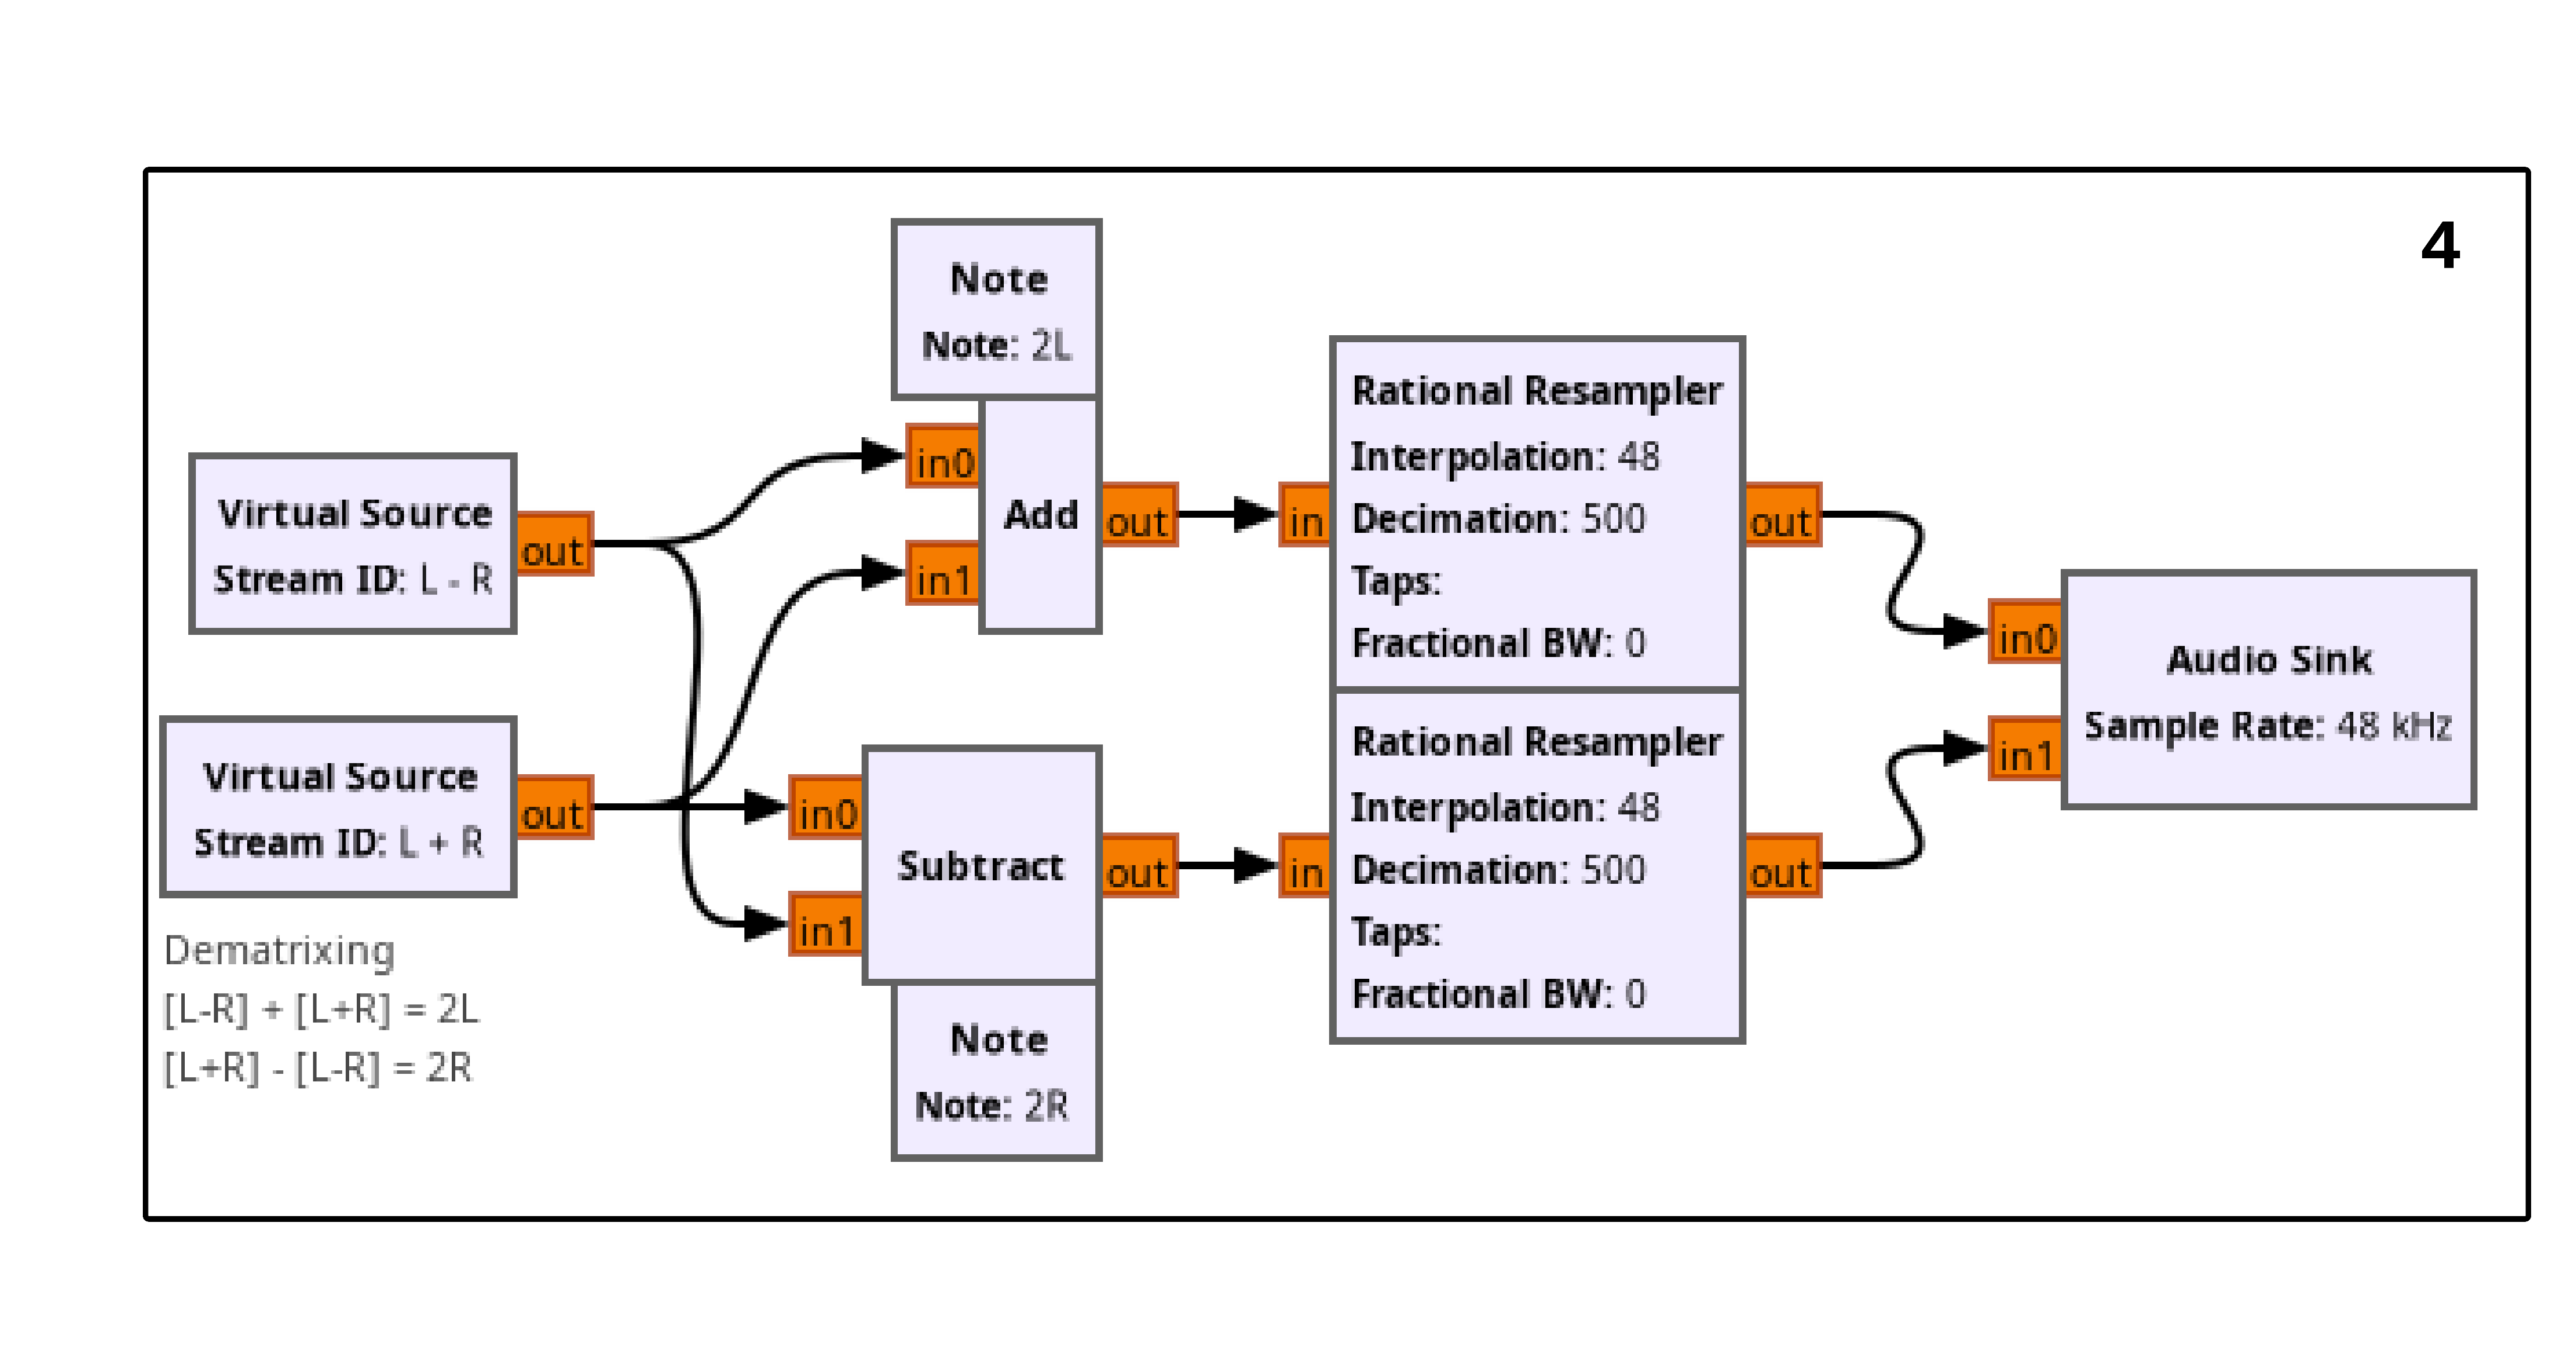
\includegraphics[width = 0.6\linewidth]{img/mods/modulo4.png}
    \caption{Recuperação dos sinais $L$ e $R$ através do processo de \textit{dematrixing}.}
    \label{fig:modulo4}
\end{figure}
%\fi

Por fim, tal como referido na introdução, a recuperação das componentes associadas ao ouvido esquerdo ($L$) e direito ($R$) do sinal é bastante trivial. Aplicando o processo de \textit{dematrixing} a $m_1(t)$ e $m_2(t)$, com auxilio dos blocos de "Add" e "Subtract" obtemos:

\begin{equation*}
  \left\{\begin{array}{@{}l@{}}
    m_1(t)+m_2(t)=2L\\
    m_1(t)-m_2(t)=2R
  \end{array}\right.\,
\end{equation*}

Contudo, é importante reparar que após este processo é essencial reduzir o ritmo amostral para $48$ kHz antes da ligação ao "Audio Sink" (reprodução do sinal de áudio). Este processo é assegurado, tal como descrito no guia, pelo bloco "Rational Resampler" em adequação com as características da placa de som do computador.